\chapter{Results}\label{cap:results}

This chapter describes the results of each stage of the framework preparation and the validation approach used to verify its applicability and effectiveness on realistic data.

\section{Tree segmentation network training results}

The results of training a tree segmentation PointNet++ are challenging to evaluate on their own because there are not inherently good metrics that would put the performance into easily understandable numbers.
As was mentioned in Section~\ref{sec-other-training-params}, during training model checkpointing is set up to track average validation accuracy – proportion of points for which the final predicted label is correct.
However, the predictions are quite noisy, resulting in low accuracies even for results that are not bad.
Figure~\ref{fig-example-prediction-2d} shows the prediction on a sample from the validation dataset used to monitor the training process, and Figure~\ref{fig-example-prediction-3d} shows the same prediction in 3D.
The accuracy of the model on the figures is 33.6\%, and it is around the best accuracy of all the experiments I ran, excluding ones with simpler data.

\begin{figure}
\centering{
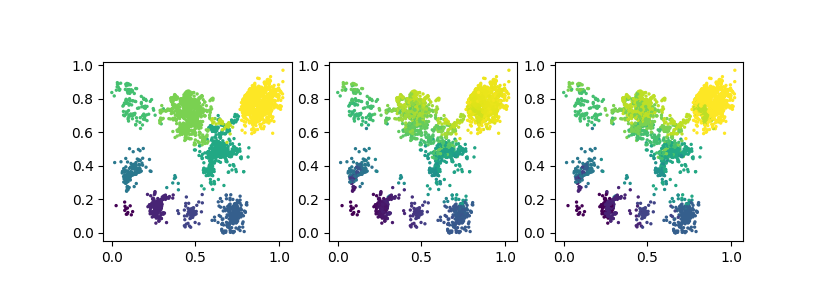
\includegraphics[width=\textwidth]{../images/example_prediction_2d.png}
}
\caption[A top-down view of an example prediction of the tree segmentation PointNet++.]{\label{fig-example-prediction-2d}A top-down view of an example
prediction of the tree segmentation PointNet++ on a sample from the
validation dataset. \textbf{Left:} Points colored by label -- tree ID
within the patch. \textbf{Middle:} Points colored by the raw prediction
of the network (the regression head outputs a continuous prediction for
every point). \textbf{Right:} Points colored by the rounded prediction
-- converted from the continuous to the final integer tree ID.}
\end{figure}

\begin{figure}
\centering{
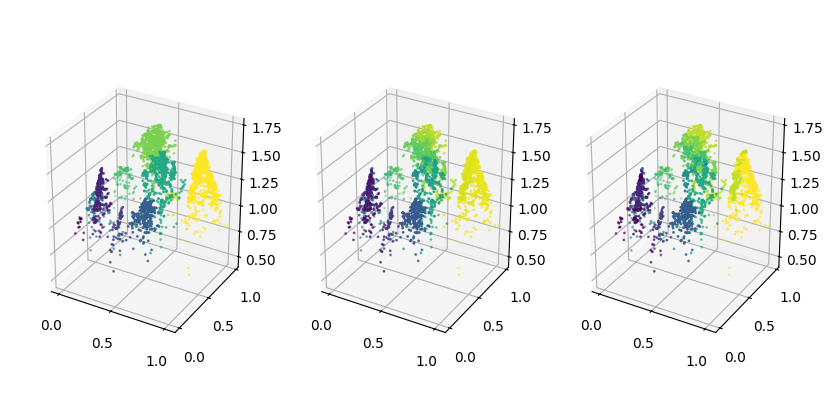
\includegraphics[width=\textwidth]{../images/example_prediction_3d.png}
}
\caption[A 3D view of an example prediction of the tree segmentation PointNet++.]{\label{fig-example-prediction-3d}A 3D view of an example
prediction of the tree segmentation PointNet++ on a sample from the
validation dataset. \textbf{Left:} Points colored by label -- tree ID
within the patch. \textbf{Middle:} Points colored by the raw prediction
of the network (the regression head outputs a continuous prediction for
every point). \textbf{Right:} Points colored by the rounded prediction
-- converted from the continuous to the final integer tree ID.}
\end{figure}

Overall, the final model was selected less based on raw numbers such as maximum average validation accuracy or minimum average validation loss, but by expecting the visualizations of the predictions on a subset of samples from the validation dataset.

\section{Attribute prediction model training results}

To evaluate the performance of the attribute prediction models, 10-fold stratified cross validation was used, as well as a separate 40\% hold-out set.
For the tree species classification model, the stratification was performed using the labels directly.
For the diameter at breast height regression model, the stratification was performed on the label split into 5 equal-width buckets across the range.

\subsubsection{Tree species classification}

The tree species classification model was evaluated using accuracy and macro $F_1$-score (an average of $F_1$-scores across all the classes).
Figure~\ref{fig-cv-clf} shows out-of-fold metrics across all ten folds of cross-validation.
The average accuracy is 0.71, with a standard deviation of 0.06.
The average macro $F_1$-score is 0.70, with a standard deviation of 0.07.
The model is overall relatively consistent across all ten folds, showing that the cross-validation metrics estimates are reliable.

\begin{figure}
\centering{
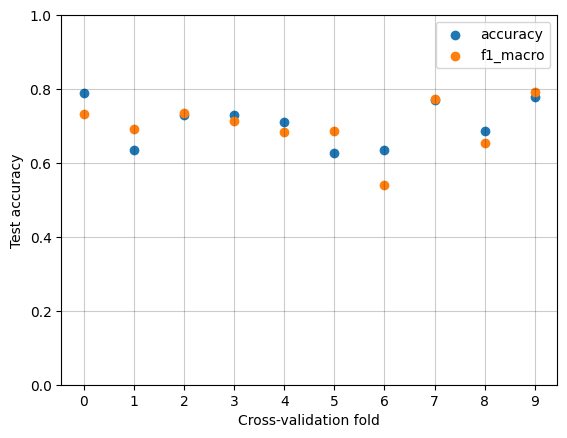
\includegraphics[width=\textwidth]{../images/train-tree-models-fig-cv-clf-output-1.png}
}
\caption[Cross-validation results of the species classification Random Forest model]{\label{fig-cv-clf}10-fold cross-validation results of the
species classification Random Forest model. The average accuracy is 0.71
with a standard deviation of 0.06. The average macro F-score is 0.70
with a standard deviation of 0.07. The model is overall stable across
all of the folds.}
\end{figure}

The holdout set was used to take a more in-depth look at the classification results.
Figure~\ref{fig-clf-confusion-matrix} shows the confusion matrix for the holdout set, with values normalized by row.
The set is relatively small – 158 examples, but enough to see some patterns emerge in the predictions.
The best overall species is spruce, and all coniferous species are better than all the deciduous species.
The model often confuses deciduous species, classifying alder as birch or tilia, aspen as birch, tilia as alder or birch.
This behavior is to be expected, as the shapes of deciduous species are very similar to each other and in complex in general.
The overall accuracy in the holdout set is 61\%.

\begin{figure}
\centering{
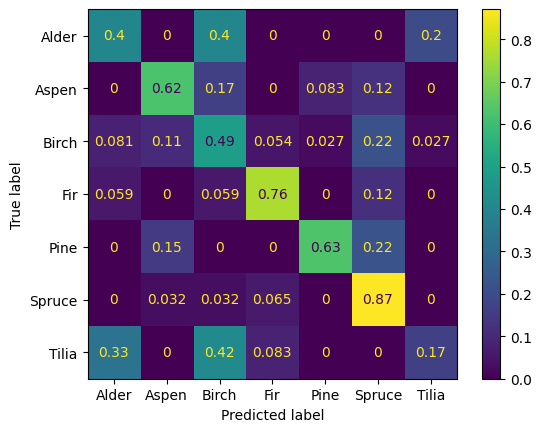
\includegraphics[width=\textwidth]{../images/train-tree-models-fig-clf-confusion-matrix-output-1.png}
}
\caption[Confusion matrix for the tree species classification Random Forest.]{\label{fig-clf-confusion-matrix}Confusion matrix for the tree
species classification Random Forest. Calulated on the 40\% holdout set
of 158 examples. Values normalized by row. The model confuses deciduous
species a lot more than coniferous ones.}
\end{figure}

\subsubsection{Diameter at breast height regression}

Diameter at breast height regression model was evaluated using root mean squared error (RMSE), mean absolute error (MAE), and coefficient of determination $R^2$.
Formulas for the metrics are provided below, with $y_i$ representing the true dbh value, $\hat y_i$ – the corresponding prediction, and $\overline y$ – the average dbh.
The dataset here is smaller than the one for tree species classification because diameter at breast height is only available for trees from the Lysva field inventory, while species are available for all trees in the individual tree point cloud dataset, some of which are from other surveys in the region.

$$
\begin{aligned}
\text{RMSE} &= \sqrt{\frac{1}{N} \sum_{i=1}^N (y_i - \hat y_i)^2} \\
\text{MAE} &= \frac{1}{N} \sum_{i=1}^N | y_i - \hat y_i | \\
R^2 &= 1 - \frac{\sum_{i=1}^N (y_i - \hat y_i)^2}{\sum_{i=1}^N (y_i - \overline y)^2}
\end{aligned}
$$


Figure~\ref{fig-cv-reg} shows out-of-fold metrics across all ten folds of cross-validation.
Both the mean squared error and the mean absolute error are stable across the folds, with average RMSE 4.55 centimeters with a standard deviation of 0.19 and average MAE 3.49 centimeters with a standard deviation of 0.38.
Coefficient of determination $R^2$ is less stable.
Even though most folds have it around 0.6 to 0.8, there are two folds where it drops to below 0.2 and even close to 0, meaning that the model there is no better than predicting the mean dbh for every input.
This drops the average $R^2$ to 0.53 with a standard deviation of 0.24.

\begin{figure}
\centering{
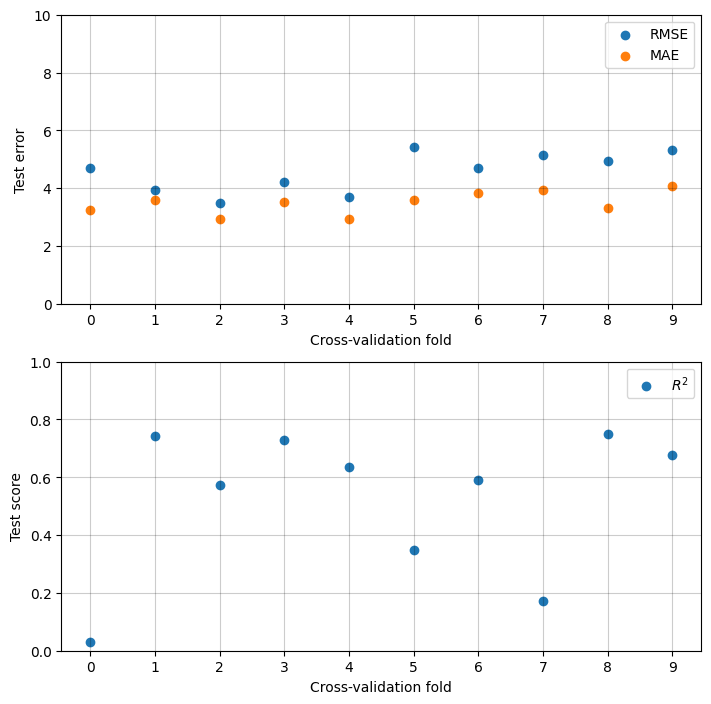
\includegraphics[width=\textwidth]{../images/train-tree-models-fig-cv-reg-output-1.png}
}
\caption[Cross-validation results of the dbh regression Random Forest model.]{\label{fig-cv-reg}10-fold cross-validation results of the dbh
regression Random Forest model. The average RMSE is 4.55 centimeters
with a standard deviation of 0.19. The average MAE is 3.49 centimeters
with a standard deviation of 0.38. The average coefficient of
determination \(R^2\) is 0.53 with a standard deviation of 0.24. The
model is relatively stable in terms of the errors, but the coefficient
of determination is all over the place.}
\end{figure}

Similar to the classification model, the holdout set was used to take a more in-depth look at the regression results.
Here the holdout set is even smaller than for regression – 68 samples.
Figure~\ref{fig-reg-residuals} offers a collection of diagnostic visualizations aimed to help better understand the regression performance.
On the top left is the residual plot, where the differences between the actual dbh and the predicted dbh are plotted against the actual dbh values.
Ideally, the points should be around a horizontal line at zero, shown in black, without any patterns.
This would mean that the size of the error does not depend on the value of dbh.
The resulting dbh regression model shows a trend, which means it tends to overestimate low dbh values and underestimate high dbh values.
A related plot is on the top right, showing the distribution of the residuals across the holdout set.
It should be centered around zero and as narrow as possible.
On the bottom left is a scatter plot of predicted dbh against the actual dbh.
Ideally, this should be a 45-degree line, shown in black.
Because of the underestimation on the high end and overestimation in the low end, the points seem to lie on a line with a smaller slope.
Although most points are in the middle, where the line is followed a lot more closely.
And, finally, a related plot on the bottom right, comparing distributions of the actual dbh and predicted dbh in the holdout set.
The same lack of extreme can be observed.
The final holdout set RMSE is 5.76 cm, MAE is 4.11, $R^2$ is 0.52.

\begin{figure}
\centering{
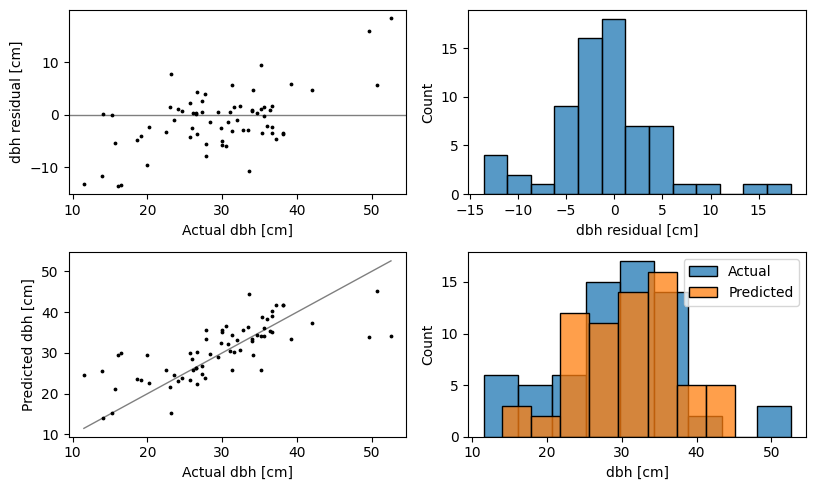
\includegraphics[width=\textwidth]{../images/train-tree-models-fig-reg-residuals-output-1.png}
}
\caption[Quality assessment plots for the dbh regression Random Forest.]{\label{fig-reg-residuals}Quality assessment plots for the
diameter at breast height regression Random Forest. Calculated on a 40\%
holdout set of 68 examples. \textbf{Top Left:} Residual scatter plot:
difference between the prediction and the true value vs.~the true value.
Ideally the spread should be equal across the valu range. \textbf{Bottom
Left:} Predicted vs.~actual scatter plot. Ideally should be as close to
a line as possible. \textbf{Top right:} Distribution of the residuals.
\textbf{Bottom right:} Distribution of the predicted and actual values
of dbh.}
\end{figure}

\section{Validation on the Lysva field inventory data}

To validate the framework, the results were evaluated on the Lysva field inventory dataset, described in Section~\ref{sec-lysva-dataset}.
The mean X and Y coordinates of each segmented tree were calculated to convert the cloud into a set of points, where each point represents a candidate detected tree.
The maximum height of the points in the cluster was used as the height of the detected tree.
Then the algorithm described in Section~\ref{sec-matching-algorithm} was applied to match the detected trees their corresponding the ground truth trees, if any.
The matching algorithm was run with maximum distance between a detected tree candidate and a ground truth tree of 5 meters and maximum height difference of 3 meters (ignored for ground truth trees that don't have measured height).
Then, precision, recall, and $F_1$-score were calculated for the detection results, and for the true positive matches the average distance between the detected tree and the actual tree, species classification accuracy and macro $F_1$-score, and diameter at breast height errors are calculated.

Table~\ref{tbl-detection-results} shows the tree detection metrics.
When interpreting the metrics, the reader is advised to keep in mind the limitations of the distance metric mentioned in Section~\ref{sec-matching-algorithm}, and instead focus on the $F_1$-score as the most informative metric.
The overall average $F_1$-score for tree detection by the described system is 0.63.
This approach thus outperforms the basic individual local maximum filter in tree detection in the Lysva region as reported in \citet{dubrovinOpenDatasetIndividual2024} by 0.13.

\begin{table}
    \centering
    \caption{Results of the tree detection across all plots in the Lysva field survey.}
    \label{tbl-detection-results}
    \begin{tabular}{lrlrrrrr}
    \toprule
     & Trees & Dominant type & Point density & Recall & Precision & $F_1$ & Distance \\
    Plot &  &  &  &  &  &  & \\
    \midrule
    1 & 420 & Deciduous & 31.7 & 0.83 & 0.63 & 0.72 & 0.77 \\
    2 & 365 & Deciduous & 47.9 & 0.61 & 0.72 & 0.66 & 0.81 \\
    3 & 332 & Deciduous & 40.3 & 0.63 & 0.49 & 0.56 & 0.85 \\
   4 & 261 & Coniferous & 33.5 & 0.85 & 0.50 & 0.63 & 1.06 \\
   5 & 208 & Coniferous & 14.2 & 0.68 & 0.55 & 0.61 & 0.97 \\
   6 & 290 & Coniferous & 39.1 & 0.80 & 0.52 & 0.63 & 0.83 \\
    7 & 408 & Deciduous & 41.9 & 0.65 & 0.62 & 0.63 & 0.85 \\
   8 & 341 & Coniferous & 35.5 & 0.87 & 0.57 & 0.69 & 0.93 \\
   9 & 459 & Coniferous & 42.1 & 0.56 & 0.65 & 0.60 & 0.92 \\
   10 & 518 & Deciduous & 42.9 & 0.42 & 0.92 & 0.58 & 0.99 \\
    \midrule
    & & & Average: & 0.69 & 0.62 & 0.63 & 0.90 \\
    \bottomrule
    \end{tabular}
\end{table}

Figure~\ref{fig-lysva-confusion-matrix} shows the confusion matrix for species prediction calculated for true positive matches.
Note that willow trees are not included, as the model has not seen any in the training data, and all pine predictions are counted as spruce instead.
The pattern of the confusion matrix is similar to the evaluation on the holdout set.
The overall accuracy is 66.1\%.
The overall macro $F_1$-score is 55.4\%.

\begin{figure}
\centering{
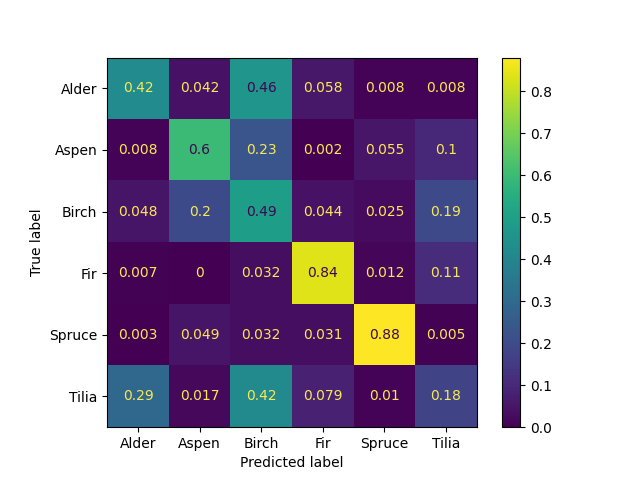
\includegraphics[width=\textwidth]{../images/lysva-confusion-matrix.png}
}
\caption[Confusion matrix for the tree species classification on true positive detected trees]{\label{fig-lysva-confusion-matrix}Confusion matrix for the tree
species classification on true positive detected trees in the Lysva
field inventory plots.}
\end{figure}

Figure~\ref{fig-lysva-regression-metrics} show the quality assessment plots for the results of diameter at breast height regression.
It's obvious from the plots that the individual tree dataset is not representative of the entire Lysva dataset in terms of dbh, as the range of dbh in there is not wide enough.
The distributions show that the individual trees dataset has higher mean dbh values than the overall distribution, which makes the model eager to overestimate a lot.
This effect is no doubt connected to the sampling bias mentioned in the description of the individual trees dataset: trees were selected by humans based on how easy they are to extract from a large point cloud.
As the result, the predictions outside the range seen by the Random Forest are constant.
Within the covered range, however, the behavior is similar to what was observed on the holdout set: a trend in the residual plot indicating over- and underestimation of low and high values, and errors close to zero near the middle of the range.
The overall root mean squared error is 5.37 centimeters.
The overall mean absolute error is 4.21 centimeters.
The overall coefficient of determination $R^2$ is 0.65.

\begin{figure}
\centering{
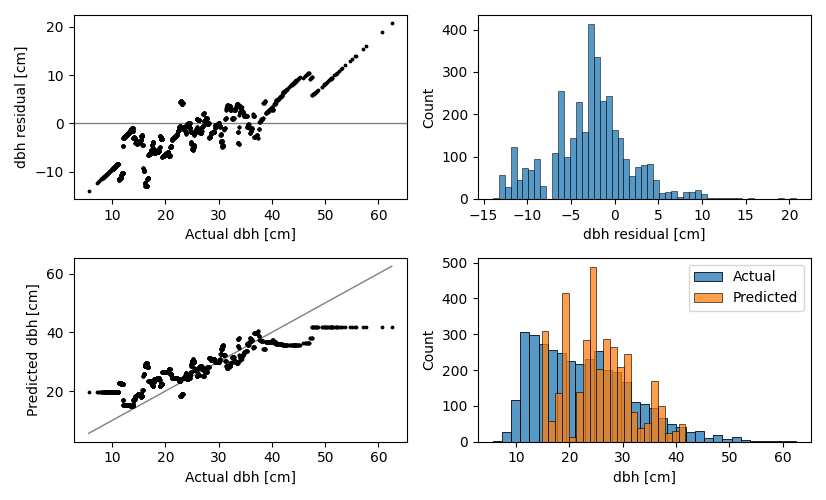
\includegraphics[width=\textwidth]{../images/lysva-regression-metrics.png}
}
\caption[Regression quality assessment plots plots for the dbh regression on true positive detected trees.]{\label{fig-lysva-regression-metrics}Regression quality
assessment plots plots for the diameter at breast height regression on
true positive detected trees in the Lysva field inventory plots.}
\end{figure}
